\documentclass[final,5p,times,twocolumn,authoryear]{elsarticle}

\usepackage{amssymb}
\usepackage{amsthm}
\usepackage{amsmath}
\usepackage[utf8]{inputenc}
\usepackage{lineno}
\usepackage{tabularx}

\newcommand{\pd}[2]{\frac{\partial #1}{\partial #2}}
\newcommand{\pdd}[2]{\frac{\partial^2 #1}{\partial #2^2}}

\journal{Graduate School@UGA}

\begin{document}

\begin{frontmatter}

\title{
\begin{minipage}{0.3\textwidth}

\includegraphics[width=0.9\textwidth]{LEGI-logo.png}
\end{minipage}%
\begin{minipage}{0.4\textwidth}
\centering
\textbf{Simulations of stratified turbulence}
\end{minipage}%
\begin{minipage}{0.3\textwidth}
\flushright

\includegraphics[width=0.9\textwidth]{UGA-logo.png}
\end{minipage}
}

\author{Guillermin Remy\\ Supervised by Pierre Augier}

\begin{abstract}
This study investigates stratified turbulence using high-resolution Direct Numerical Simulations (DNS).
\end{abstract}

\begin{keyword}
%% keywords here, in the form: keyword \sep keyword, up to a maximum of 6 keywords
Numerical Simulation \sep Fluids Dynamic \sep Turbulence

\end{keyword}

\end{frontmatter}

\section{Introduction}
\label{introduction}

In fluid mechanics, turbulence arises for large Reynolds number, $\mathrm{Re} = UL/\nu$, where $U$ and $L$ are the characteristic velocity and length scales of the flow, and $\nu$ is the kinematic viscosity. This condition is typically met in scenarios such as high-speed flows (e.g., jet engine exhaust), large-scale flows (e.g., atmospheric or ocean currents), or in fluids with negligible viscosity, like superfluids. Turbulence is characterised by chaotic, irregular motion that significantly affects the transport of momentum, heat, and mass.

In the context of large-scale climate systems, such as the ocean and atmosphere, turbulence is even more complex due to the additional influence of Earth’s rotation and the density stratification due to temperature (in the atmosphere) or/and salinity gradients (in the ocean). These factors modify the basic dynamics described by the Navier-Stokes equations. Specifically, stratification leads to the formation of internal waves, which in turn interact with turbulence in intricate ways, driving the transport and mixing processes that are fundamental to climate dynamics.

This project focuses on the effects of density stratification in large-scale flows, particularly how it induces internal wave turbulence. Understanding this phenomenon is crucial because internal waves play a key role in energy transfer within oceans and atmospheres, influencing ocean currents and atmospheric circulation patterns. By studying turbulent flows under stratified conditions, we aim to gain insights into the mechanisms governing large-scale climate dynamics and the energy cascades that drive these systems.

In a first part we will focus on the theory about such flows, we will study the wave in stratified and rotating flows but in our simulation we will only cover the stratified case.

In a second part we will describe the issues faced, how they have been resolved. We will also talk about the simulation parameters.

Finally in the last part we will discuss the results obtained for different simulation. 

\section{Theoretical background}
\subsection{Navier-Stokes Equations}

The governing equations for fluid motion in this study are the Navier-Stokes equations, given by:
\begin{subequations}
\begin{align}
\pd{\rho}{t} + \vec{\nabla} \left( \rho \vec{u} \right) &= 0 \\
\rho \left( \pd{\vec{u}}{t} + \left( \vec{u} \cdot \vec{\nabla} \right) \vec{u} \right) &= - \vec{\nabla} p - \rho g \hat{z} + \mu \Delta \vec{u} - 2 \rho \vec{\Omega} \wedge \vec{u}
\end{align}
\label{eq:NS}
\end{subequations}
where $\rho$ is the fluid density, $\vec{u}$ is the velocity field, $p$ is the pressure, $\mu$ is the dynamic viscosity, $\vec{\Omega}$ is the rotation of the frame of reference and $g$ is the acceleration due to gravity. These equations describe the motion of a viscous fluid, accounting for both inertial and gravitational forces.

\subsection{Dimensionless Numbers}

In the study of fluid mechanics, the Froude number $\mathrm{Fh}$ is a key dimensionless quantity that represents the ratio of inertial forces (advection) to gravitational forces.
\begin{equation*}
	\mathrm{Fr}^2 = U^2 / gH
\end{equation*} 
Here, $U$ is the characteristic velocity, $g$ is gravitational acceleration, and $H$ is the characteristic depth or length scale of the flow. The Froude number is useful in understanding the behaviour of stratified fluids, where gravity plays a significant role in the dynamics.

The Richardson number $Ri$ is a key parameter that characterizes the ratio of buoyancy forces to flow shear forces [\cite{cushman-roisin_introduction_2011}]. This dimensionless number is defined as:
\begin{equation}
Ri = \frac{N^2}{\left(d \bar{u} / dz \right)^2}
\end{equation}

Where $N^2 = -\frac{g}{\rho} \pd{\rho}{z}$ is the Brunt-Väisälä frequency [\cite{pedlosky_geophysical_1979}] and $d \bar{u} / dz$ is the vertical velocity gradient.

For rotating flow we can also define the Rossby number as the ratio of the inertial forces and the Coriolis forces
\begin{equation*}
	Ro = \frac{U}{fL}
\end{equation*}
Here, $f$ is the Coriolis parameter $f = 2\Omega$ in the case of a planar frame of reference, if we look at the case of the Earth, we need to take account of the latitude at which the experiment/simulation takes place.

\subsection{Boussinesq Approximation and Inertia-Wave Propagation}

For density stratified fluids, the Boussinesq approximation [\cite{boussinesq_theorie_1897}] is commonly applied, which assumes that density variations are small and only affect the buoyancy force, while the density is constant elsewhere. After applying this approximation to the Navier-Stokes equations and simplifying, we derive the gravity-wave propagation equation:
\begin{equation}
\partial^2_t \vec{u} = \left( N^2 \nabla^2_h \nabla^{-2} \right) \vec{u} \label{eq:Wave Propagation}
\end{equation}
where $\nabla_h$ is the horizontal gradient operator, $\nabla$ is the spatial gradient operator, and $N$ is the Brunt-Väisälä frequency. This equation describes the propagation of internal waves in a stratified fluid.

\subsection{Dispersion Relation of Gravity Waves}

The dispersion relation for inertia-gravity waves is given by:
\begin{equation}
\omega^2 = \frac{f^2 k_z^2 + N^2 k_h^2}{k^2} \label{eq:Dispersion relation}
\end{equation}
where $\omega$ is the frequency of the wave, $k_z$ is the vertical wave-vector and $k_h^2 = k_x^2 + k_y^2$ is the horizontal wave-vector. This relation shows that the frequency $\omega_+$ is bounded within the range $\left[ f, N \right]$ and $\omega_-$ between $\left[ N, -f \right]$, where $N$ is the Brunt-Väisälä frequency, which determines the stability of stratified fluid systems and $f$ is the Coriolis frequency, which quantifies the rotation of the frame of reference.

\section{Numerical Setup}

\subsection{Computational Tools}

This study leverages \texttt{Fluidsim} [\cite{fluiddyn}], a high-performance computing (HPC) code utilizing pseudo-spectral solvers. \texttt{Fluidsim} is particularly well-suited for simulating fluid dynamics in stratified flows, offering efficient computation for large-scale simulations.

\subsection{Computational Environment}

The simulations will be performed on two platforms. Through the master’s program, we have access to the Zen supercomputer hosted by Mesonet. This cluster was straightforward to begin working with, as it has been used in several courses and was sufficient for running low-resolution simulations to test and validate the simulation scripts. However, we encountered difficulties in utilizing parallelization effectively on this cluster, which limited its potential for larger simulations.

The second platform is the Dahu cluster, hosted by GRICAD at LEGI. This cluster offers multiple options for software installation. The first option involves using a \texttt{miniforge} environment, which is relatively simple to set up. This environment allows for single-node parallelization on the cluster, enabling simulations up to a resolution of $(256, 256, 64)$. The second option is to use \texttt{Guix}, which provides multi-node capabilities essential for performing high-resolution simulations. Unfortunately, we were unable to fully configure the multi-node setup within the \texttt{Guix} installation, limiting our ability to leverage the cluster’s full computational capacity.

\subsection{Challenges Encountered}

Several technical challenges impacted the simulation workflow.

On the Zen cluster, we were unable to configure its parallelization capabilities, restricting us to sequential simulations. This significantly reduced computational efficiency, particularly for high-resolution cases.

Additionally, while \texttt{Fluidsim} provides job submission commands for multi-node parallelization, misconfigurations prevented us from fully utilizing this feature, leading to inefficient simulations.

Another issue arose when saving physical fields with \texttt{h5py} during parallel simulations. The resulting corrupted files were unusable, an issue now identified and expected to be resolved by using the standard \texttt{h5py} library.

Addressing these challenges is crucial for enabling efficient high-resolution Direct Numerical Simulations (DNS) and should be a priority for future work. For now, we will focus on simulations using the \texttt{miniforge} installation on the GRICAD cluster, as it currently provides the most reliable and efficient computational environment.

\section{Simulation Parameters}

\subsection{Direct Numerical Simulation (DNS) Requirements}

Direct Numerical Simulations (DNS) require high grid resolutions capable of resolving all turbulent scales down to the Kolmogorov length scale $\eta$. This ensures the accurate representation of flow dynamics across the entire spectrum, from large-scale eddies to fine-scale dissipation. 


\subsection{Reynolds Number and viscosity}

The Reynolds number  $Re_n$  for a viscosity of order n is expressed as:
\begin{equation*}
Re_n = \frac{U L^{n-1}}{\nu_n}
\end{equation*}
where  $\nu_n$ represents the viscosity of order  n . For  $n = 2$ ,  $\nu_2$  corresponds to the standard viscosity term from the Navier-Stokes equations. For  $n > 2$ , higher-order viscosities (\textit{hyperviscosities}) appear as dissipation terms of the form  $\nu_n \nabla^n$ , providing flexibility for controlling dissipation at small scales but at the expense of losing DNS fidelity.

\subsection{Turbulent Scaling and Kolmogorov Length Scale}

For $n = 2$, using the turbulent scaling  $u(l) = (\varepsilon l)^{1/3}$, the Reynolds number at a length scale $l$ becomes:
\begin{equation*}
Re(l) = \frac{\varepsilon^{1/3} l^{4/3}}{\nu}
\end{equation*}

The Kolmogorov length scale $\eta$, defined as the scale where  $Re(l) = 1$, is:
\begin{equation*}
\eta = \left(\frac{\nu}{\varepsilon^{1/3}}\right)^{3/4}
\end{equation*}

Assuming  $\nu_2 = 10^{-6}$ and $\varepsilon = 1$, the Kolmogorov length scale  $\eta_2$  is approximately  $10^{-4.5}$ . This would necessitate a horizontal resolution of  $n_x \approx 30,198$  grid points, which is computationally unfeasible for this project.

We will choose $\eta$ so that we have $k_{max} \eta \sim 0.5$ which allows us to have a bigger inertial range while having almost a DNS.

We can then compute the required viscosity,
\begin{equation*}
\nu = \eta^{4/3} \varepsilon^{1/3}
\end{equation*}

In our case, this gives us $\nu = 2.296 \times 10^{-4}$. This value of viscosity ensures that turbulence is adequately resolved in our simulation, allowing us to analyze its dynamics effectively.

\section{Simulation Results}
\subsection{Isotropic Test Case}

To validate the basic behavior of isotropic turbulence, we perform simulations on a grid resolution of $(256 \times 256 \times 64)$ without stratification. This serves as a reference case to ensure that the solver correctly reproduces turbulent dynamics before introducing stratification effects.

For this, we use the standard 3D solver from \texttt{Fluidsim}, \texttt{fluidsim.solvers.ns3d}, which solves the incompressible Navier-Stokes equations using a pseudo-spectral method:
\begin{equation*}
\partial_t \textbf{v} + \textbf{v} \cdot \boldsymbol{\nabla} \textbf{v} =
- \boldsymbol{\nabla} p  + \nu \Delta \textbf{v},
\end{equation*}
where $\textbf{v}$ is the velocity field, $p$ is the pressure, and $\nu$ is the kinematic viscosity.

This solver allows for different forcing schemes and initial conditions. Here, we apply a random isotropic forcing within a spectral range of $(k_{\min}, k_{\max}) = (3,4)$ with a low amplitude to generate turbulence. 

This simulation also serves as the $N=0.0$ case in our stratified turbulence study, providing a baseline for comparison. Additionally, it allows us to test and validate our analysis tools in \texttt{jupyter} notebooks before processing more complex simulations.

\subsection{Simulation parameters}
The simulation parameters for our simulations are summarized in Table \ref{Table1}. 
\begin{table}[h]
\centering
\renewcommand{\arraystretch}{1.5}
\begin{tabular}{l c c c c c} 
 \hline
 Name  & $Fh$ & $n_z$ & T & $\tau$ & $k_{\text{max}} \eta$ \\
 \hline \hline
 ns3d-00 & $\infty$ & $64$ & 315 & 60 & 0.8\\
 ns3d-01 & 10 & $64$ & 298 & 40 & 0.5 \\
 ns3d-02 & 5 & $64$ & 278 & 40 & 0.5 \\
 ns3d-05 & 2 & $64$ & 290 & 40 & 0.5 \\
 ns3d-1 & 1 & $64$ & 286 & 40 & 0.5 \\
 ns3d-2 & 0.5 & $64$ & 275 & 40 & 0.5 \\
 ns3d-5 & 0.2 & $64$ & 270 & 40 & 0.5 \\
 ns3d-10 & 0.1 & $64$ & 210 & 40 & 0.5 \\ 
 ns3d-20 & 0.05 & $64$ & 255 & 40 & 0.5 \\ 
 \hline
\end{tabular}
\caption{Simulation parameters for the stratified dataset. T is the computing time (minutes), $\tau$ is the physical simulation time.\label{Table1}}
\end{table}

\subsubsection{Physical Space Representations}

At the end of the simulation, we analyze the velocity field by plotting the magnitude or individual components of the velocity. Figure \ref{fig:iso slice} shows the velocity magnitude in an arbitrary horizontal slice of the computational domain.
\begin{figure}[h]
\centering
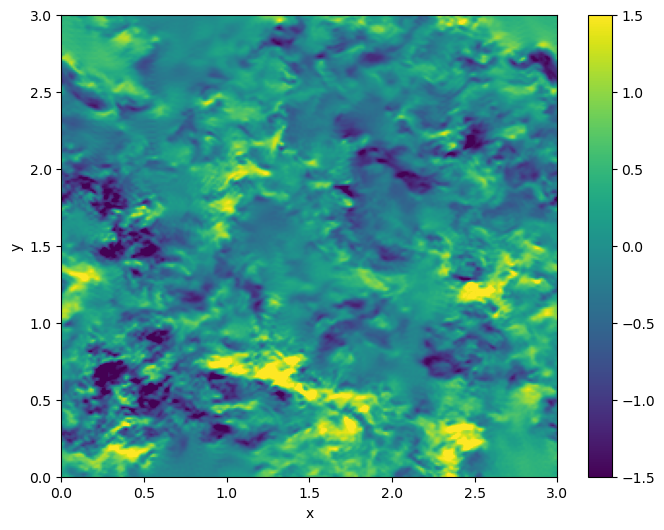
\includegraphics[width=0.4\textwidth]{fig/iso_slice.png}
\caption{Velocity magnitude in a horizontal slice.}
\label{fig:iso slice}
\end{figure}

To ensure the incompressibility of the flow, we compute the divergence of the velocity field with a \texttt{numpy.gradient} and find out that other than few artefacts due to the gradient 

The results confirm that the flow is nearly divergence-free, as expected for an incompressible flow.

\subsubsection{Spectra}
Alongside the physical fields, the solver also saves spectral data for post-processing. This includes both one-dimensional and three-dimensional spectral information as well as the spectral energy budget over time.

We plot the evolution of the spectral energy budget over time in Figure \ref{fig:iso budget}. 
\begin{figure}[h]
	\centering
	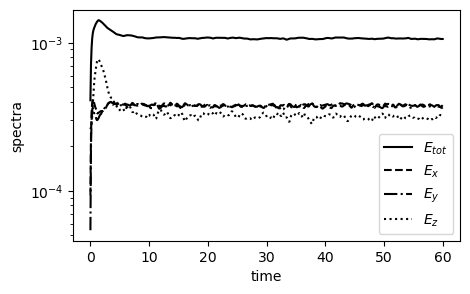
\includegraphics[width=0.45\textwidth]{fig/iso_budget.png}
	\caption{Energy budget along each direction for the isotropic case.} 
	\label{fig:iso budget}
\end{figure}

The results show a uniform distribution of energy across the three spatial directions, with a slight deficit in the vertical direction which is attributed to the reduced vertical scale.

\subsection{Ensemble analysis}

We conducted simulations using the solver \texttt{fluidsim.solvers.ns3d.strat}, varying the Brunt-Väisälä frequency $N$ across different cases.

This solver solves the Navier-Stokes equations of the velocity $\textbf{v}$ and the buoyancy $b$ under the Boussinesq approximation with a constant Brunt-Väisälä frequency
\begin{align*}
	\partial_t \textbf{v} + \textbf{v} \cdot \boldsymbol{\nabla} \textbf{v} & = - \boldsymbol{\nabla} p + b \textbf{e}_\textbf{z} + \nu \Delta \textbf{v} \\
    \partial_t b  + \textbf{v} \cdot \boldsymbol{\nabla} b & = - N^2 v_z + \nu \Delta b
\end{align*}

The Brunt-Väisälä frequency $N$ in each simulation is characterized by its corresponding Froude number, defined as:
\begin{equation*}
    Fh = \frac{U}{NL} = \frac{\varepsilon^{1/3}}{N L^{2/3}} = \frac{1}{N}
\end{equation*}

We apply a random forcing with the same characteristics as in the non-stratified case, maintaining consistency across simulations.

\subsubsection{Spectra}

When examining the spectral budget for highly stratified cases, we observe that vertical energy rapidly decreases to values lower than the horizontal energy. This highlights the impact of stratification on energy budget. Additionally, after less than five seconds, most cases reach a stable state, allowing us to compute the mean energy ratio between horizontal and vertical directions.

The horizontal energy spectrum for each simulation is shown in Figure \ref{fig:multi spectrum}, along with the theoretical inertial range slope $E(k) \propto k^{-5/3}$.

\begin{figure}[h]
\centering
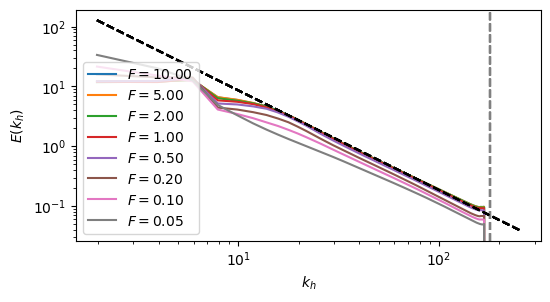
\includegraphics[width=0.5\textwidth]{fig/multi_Ekh_kh.png}
\caption{Horizontal energy spectrum for the stratified cases. The dashed line represents the inertial range slope $E(k) \propto k^{-5/3}$, while the vertical line marks the dissipation range.}
\label{fig:multi spectrum}
\end{figure}

Despite the resolution limitations, we observe a well-defined inertial range that follows the expected $E(k) \propto k^{-5/3}$ scaling. However, with $k_{\max} \eta = 0.5$, the dissipation range is somewhat suppressed. A slightly higher value, such as $0.8$, may better capture the small-scale dissipation.

As the Froude number decreases—i.e., as the Brunt-Väisälä frequency increases—the energy spectrum shifts downward, further illustrating the effect of stratification on turbulence dynamics.


\section{Discussion}

This master’s project investigated stratified turbulence using simulations on HPC systems. While high-resolution simulations up to $(1024, 1024, 256)$ were not achieved due to unresolved parallelization issues, lower-resolution runs provided valuable insights.

The results illustrate how increasing stratification suppresses vertical energy dissipation and enhances horizontal dynamics. These findings align with theoretical expectations and emphasize the anisotropic nature of stratified turbulence. Addressing the computational challenges and conducting higher-resolution simulations should be a key focus for future work to refine these observations further.

\appendix

\section{Bibliography}

\bibliographystyle{elsarticle-harv} 
\bibliography{references.bib}

\section{Figures}

\begin{figure}[h]
	\centering
	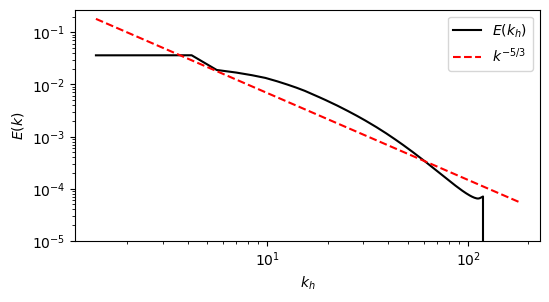
\includegraphics[width=0.45\textwidth]{fig/iso_Ekh_kh.png}
	\caption{Horizontal energy spectrum for the non stratified case. The dashed line indicates the inertial range slope $E(k) \propto k^{-5/3}$. } 
	\label{fig:iso horizontal spectrum}
\end{figure}

\begin{figure}[h]
	\centering
	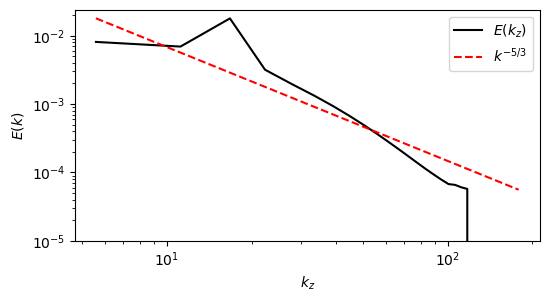
\includegraphics[width=0.45\textwidth]{fig/iso_Ekz_kz.png}
	\caption{Vertical energy spectrum for the non stratified case. The dashed line indicates the inertial range slope $E(k) \propto k^{-5/3}$. } 
	\label{fig:iso vertical spectrum}
\end{figure}

\begin{figure}[h]
	\centering
	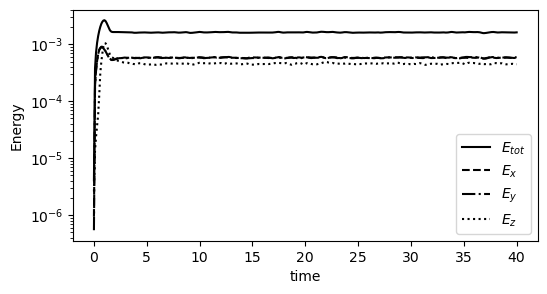
\includegraphics[width=0.45\textwidth]{fig/0.5_budget.png}
	\caption{Energy budget along each direction for the case with $N=0.5$} 
	\label{fig:0.5 budget}
\end{figure}

\begin{figure}[h]
	\centering
	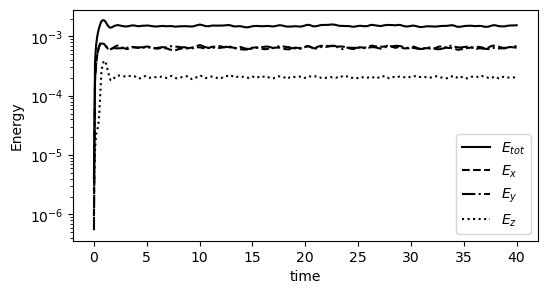
\includegraphics[width=0.45\textwidth]{fig/10_budget.png}
	\caption{Energy budget along each direction for the case with $N=10$} 
	\label{fig:10 budget}
\end{figure}

\begin{figure}[h]
	\centering
	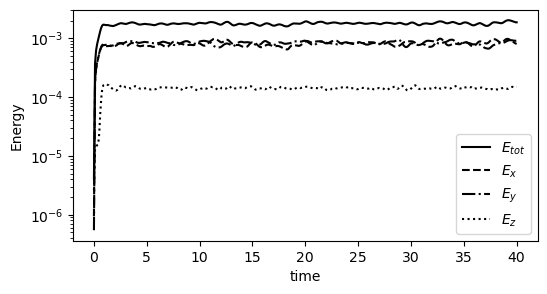
\includegraphics[width=0.45\textwidth]{fig/20_budget.png}
	\caption{Energy budget along each direction for the case with $N=20$} 
	\label{fig:20 budget}
\end{figure}

\begin{figure}[h]
	\centering
	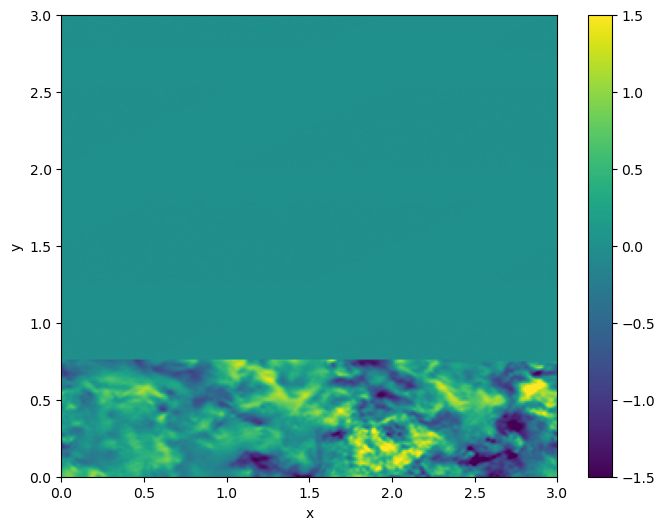
\includegraphics[width=0.45\textwidth]{fig/corrupt_slice.png}
	\caption{Slice of a corrupted file} 
	\label{fig:corrupt}
\end{figure}



\begin{figure}[h]
\centering
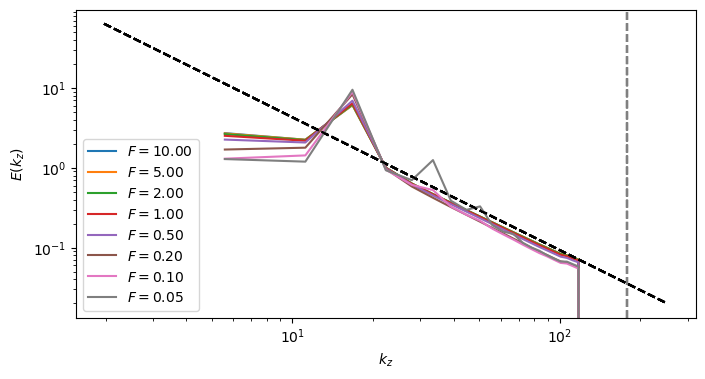
\includegraphics[width=0.45\textwidth]{fig/multi_Ekz_kz.png}
\caption{Vertical energy spectrum for the stratified cases. The dashed line indicates the inertial range slope $E(k) \propto k^{-5/3}$. The vertical line is the dissipation range.}
\label{fig:multi vertical spectrum}
\end{figure}

\end{document}

\endinput